\documentclass[11pt,]{book}
\usepackage{lmodern}
\usepackage{amssymb,amsmath}
\usepackage{ifxetex,ifluatex}
\usepackage{fixltx2e} % provides \textsubscript
\ifnum 0\ifxetex 1\fi\ifluatex 1\fi=0 % if pdftex
  \usepackage[T1]{fontenc}
  \usepackage[utf8]{inputenc}
\else % if luatex or xelatex
  \ifxetex
    \usepackage{mathspec}
  \else
    \usepackage{fontspec}
  \fi
  \defaultfontfeatures{Ligatures=TeX,Scale=MatchLowercase}
    \setmainfont[]{Calibri}
\fi
% use upquote if available, for straight quotes in verbatim environments
\IfFileExists{upquote.sty}{\usepackage{upquote}}{}
% use microtype if available
\IfFileExists{microtype.sty}{%
\usepackage{microtype}
\UseMicrotypeSet[protrusion]{basicmath} % disable protrusion for tt fonts
}{}
\usepackage[margin=1in]{geometry}
\usepackage{hyperref}
\PassOptionsToPackage{usenames,dvipsnames}{color} % color is loaded by hyperref
\hypersetup{unicode=true,
            pdftitle={Ontwerp van een early-warning meetnet voor droogte in natuurgebieden},
            pdfauthor={Jan Wouters, Floris Vanderhaeghe},
            colorlinks=true,
            linkcolor=link.colour,
            citecolor=link.colour,
            urlcolor=link.colour,
            breaklinks=true}
\urlstyle{same}  % don't use monospace font for urls
\usepackage{longtable,booktabs}
\usepackage{graphicx,grffile}
\makeatletter
\def\maxwidth{\ifdim\Gin@nat@width>\linewidth\linewidth\else\Gin@nat@width\fi}
\def\maxheight{\ifdim\Gin@nat@height>\textheight\textheight\else\Gin@nat@height\fi}
\makeatother
% Scale images if necessary, so that they will not overflow the page
% margins by default, and it is still possible to overwrite the defaults
% using explicit options in \includegraphics[width, height, ...]{}
\setkeys{Gin}{width=\maxwidth,height=\maxheight,keepaspectratio}
\IfFileExists{parskip.sty}{%
\usepackage{parskip}
}{% else
\setlength{\parindent}{0pt}
\setlength{\parskip}{6pt plus 2pt minus 1pt}
}
\setlength{\emergencystretch}{3em}  % prevent overfull lines
\providecommand{\tightlist}{%
  \setlength{\itemsep}{0pt}\setlength{\parskip}{0pt}}
\setcounter{secnumdepth}{5}
% Redefines (sub)paragraphs to behave more like sections
\ifx\paragraph\undefined\else
\let\oldparagraph\paragraph
\renewcommand{\paragraph}[1]{\oldparagraph{#1}\mbox{}}
\fi
\ifx\subparagraph\undefined\else
\let\oldsubparagraph\subparagraph
\renewcommand{\subparagraph}[1]{\oldsubparagraph{#1}\mbox{}}
\fi

%%% Use protect on footnotes to avoid problems with footnotes in titles
\let\rmarkdownfootnote\footnote%
\def\footnote{\protect\rmarkdownfootnote}

%%% Change title format to be more compact
\usepackage{titling}

% Create subtitle command for use in maketitle
\providecommand{\subtitle}[1]{
  \posttitle{
    \begin{center}\large#1\end{center}
    }
}

\setlength{\droptitle}{-2em}

  \title{Ontwerp van een early-warning meetnet voor droogte in natuurgebieden}
    \pretitle{\vspace{\droptitle}\centering\huge}
  \posttitle{\par}
    \author{Jan Wouters, Floris Vanderhaeghe}
    \preauthor{\centering\large\emph}
  \postauthor{\par}
      \predate{\centering\large\emph}
  \postdate{\par}
    \date{Versie 2019-11-18 19:47:56}

% definition of INBO colours
\RequirePackage{xcolor}
\definecolor{box.colour}{RGB}{229, 229, 229}
\definecolor{link.colour}{RGB}{192, 67, 132}

% allow landscape pages and define commands that work with pandoc
\RequirePackage{lscape}
\newcommand{\blandscape}{\begin{landscape}}
\newcommand{\elandscape}{\end{landscape}}

% allow use of FloatBarrier
\RequirePackage{placeins}

% definition of block, alertblock and exampleblock
\RequirePackage{mdframed}

\newenvironment{block}[2][]{%
  \begin{mdframed}[backgroundcolor=box.colour]
  \textbf{#2}%

}
{
  \end{mdframed}
}
\usepackage{booktabs}
\usepackage{longtable}
\usepackage{array}
\usepackage{multirow}
\usepackage{wrapfig}
\usepackage{float}
\usepackage{colortbl}
\usepackage{pdflscape}
\usepackage{tabu}
\usepackage{threeparttable}
\usepackage{threeparttablex}
\usepackage[normalem]{ulem}
\usepackage{makecell}
\usepackage{xcolor}

\begin{document}
\maketitle

{
\hypersetup{linkcolor=black}
\setcounter{tocdepth}{2}
\tableofcontents
}
\chapter{Inleiding}\label{inleiding}

\begin{quote}
Het basisidee van het early-warning meetnet droogte is om in
natuurgebieden een vooraf gekozen aantal meetpunten zo goed mogelijk
ruimtelijk gebalanceerd te selecteren, rekening houdende met mogelijke
verschillen in het gedrag van het grond/oppervlaktewaterpeil t.a.v. een
neerslagtekort. Voor deze meetpunten kan op basis van actuele informatie
een indicator (cfr. droogte-indicator) worden berekend.
\end{quote}

Het project omhelst :

\begin{itemize}
\tightlist
\item
  uitwerking van een methodiek die een ruimtelijk gebalanceerde selectie
  van actuele en potentiële meetlocaties mogelijk maakt
\item
  bepalen van referentiewaarden voor de actuele meetlocaties
\end{itemize}

Met natuurgebieden worden hier alle locaties met grondwaterafhankelijke
habitattypes en rbb's bedoeld, gelegen binnen of buiten het Natura 2000
netwerk. In overeenstemming met het meetnet natuurlijk milieu (MNM) voor
de milieudruk `verdroging via grondwater' worden volgende habitattypen
en rbb's als grondwaterafhankelijk beschouwd (tabel \ref{tab:gw-typen}).
Hierna worden deze typen afgekort tot gaHT.

\begin{table}

\caption{\label{tab:gw-typen}grondwaterafhankelijke habitattypen en rbb's}
\centering
\begin{tabular}[t]{l|l|r}
\hline
habitat(sub)type of rbb & (verkorte) naam & GT-groep: nummer\\
\hline
1310\_pol & binnendijkse zeekraalvegetatie & 3\\
\hline
1310\_zk & buitendijks laag schor & 1\\
\hline
1310\_zv & buitendijks hoog schor & 1\\
\hline
1320 & schorren met slijkgras & 1\\
\hline
1330\_da & buitendijkse schor & 1\\
\hline
1330\_hpr & zilte graslanden & 3\\
\hline
2130\_had & kalkarme duingraslanden & 5\\
\hline
2130\_hd & kalkrijke duingraslanden & 5\\
\hline
2160 & duindoornstruwelen & 4\\
\hline
2170 & kruipwilgstruwelen & 4\\
\hline
2180 & duinbossen & 4\\
\hline
2190\_mp & duinpannen (kalkrijk) & 2\\
\hline
2190\_overig & vochtige duinvalleien - overige vegetaties & 4\\
\hline
3270 & voedselrijke slikoevers met bepaalde eenjarige planten & 1\\
\hline
4010 & vochtige heide & 3\\
\hline
6230\_hmo & vochtige heischrale graslanden & 4\\
\hline
6410\_mo & blauwgrasland & 3\\
\hline
6410\_ve & veldrusgrasland & 3\\
\hline
6430\_bz & nitrofiele boszoom & 5\\
\hline
6430\_hf & moerasspirearuigte & 3\\
\hline
6430\_hw & ruigte en zoom met harig wilgenroosje & 3\\
\hline
6430\_mr & ruiger rietland & 2\\
\hline
6510\_hua & habitatwaardig vossenstaartgrasland & 4\\
\hline
6510\_hus & pimpernelgrasland & 4\\
\hline
7140\_base & basenrijk trilveen & 1\\
\hline
7140\_meso & circum-neutraal overgangsveen & 1\\
\hline
7140\_mrd & rietland op drijftillen & 1\\
\hline
7140\_oli & zuur overgangsveen & 1\\
\hline
7150 & pioniervegetaties met snavelbiezen & 3\\
\hline
7210 & galigaanmoerassen & 1\\
\hline
7230 & alkalisch laagveen & 1\\
\hline
9130\_end & atlantisch neutrofiel beukenbos & 4\\
\hline
9130\_fm & midden-Europese neutrofiel beukenbos & 5\\
\hline
9160 & eiken-haagbeukenbossen & 4\\
\hline
9190 & oude eiken-berkenbossen & 5\\
\hline
91E0\_sf & wilgenvloedbos & 3\\
\hline
91E0\_va & beekbegeleidend bos & 4\\
\hline
91E0\_vc & goudveil-essenbos & 1\\
\hline
91E0\_vm & mesotroof broekbos & 1\\
\hline
91E0\_vn & ruigt-elzenbos & 3\\
\hline
91E0\_vo & oligotroof broekbos & 1\\
\hline
91F0 & hardhoutooibossen & 4\\
\hline
rbbhc & dotterbloemgrasland & 3\\
\hline
rbbhf & moerasspirearuigte met graslandkenmerken & 3\\
\hline
rbbhfl & natte ruigte met grote wederik en hennegras & 3\\
\hline
rbbkam & kamgrasland & 5\\
\hline
rbbmc & grote zeggenvegetatie & 2\\
\hline
rbbmr & rietland en andere vegetatie van het rietverbond & 2\\
\hline
rbbms & kleine zeggenvegetatie niet vervat in 7140 & 2\\
\hline
rbbppm & structuurrijk, oud bestand van grove den & 5\\
\hline
rbbsf & moerasbos van breedbladige wilgen & 3\\
\hline
rbbsm & gagelstruweel & 3\\
\hline
rbbso & vochtig wilgenstruweel op venige of zure grond & 3\\
\hline
rbbvos & grote vossenstaartgrasland & 4\\
\hline
rbbzil & zilverschoongrasland & 3\\
\hline
\end{tabular}
\end{table}

Een min of meer ruimtelijk gebalanceerde set van bestaande meetlocaties
maakt het mogelijk om conclusies te trekken die benaderend
representatief zijn voor heel het studiegebied. Via deze benadering
wordt ook een goede synergie bekomen met de implementatie van de zg.
`overgangsfase' van het grondwatermeetnet in MNM (Vanderhaeghe \emph{et
al.}, \protect\hyperlink{ref-vanderhaeghe_meetnetten_2018}{2018}:
hoofdstuk 6).

Er wordt met dit meetnet niet beoogd om specifiek voor elk gaHT te
bepalen of het aan droogte onderhevig is. Het meetnet wil een globale
uitspraak faciliteren. Hierbij achten we het belangrijk om rekening te
houden met de mogelijke verschillen in responstijd (`hoe snel laat een
neerslagtekort zich voelen in een wijziging van het grondwaterpeil') op
droogte. De responstijd is onder meer afhankelijk van de
landschappelijke positie. Vegetaties die voorkomen in
lokaal-grondwatergevoede systemen zullen sneller een droogte gewaar
worden dan vegetaties die gebonden zijn aan (regionale) systemen met een
permanente aanvoer van grondwater. We veronderstellen hierbij dat er een
relatie bestaat tussen het hydrologisch regime en de responstijd:
permanent grondwatergevoede systemen reageren trager dan systemen met
een tijdelijke of zwakke grondwatervoeding.

We vertrekken hiervoor van de 5-delige indeling in grondwatertypegroepen
(GT-groep) die toegepast wordt in het MNM (tabel \ref{tab:GTgroepen}).
In de vorige tabel \ref{tab:gw-typen}) is weergegeven tot welke GT-groep
een gaHT gerekend wordt.

\begin{table}

\caption{\label{tab:GTgroepen}Grondwatertype-groepen}
\fontsize{9}{11}\selectfont
\begin{tabu} to \linewidth {>{\raggedleft}X>{\raggedright}X}
\hline
GT-groep: nummer & GT-groep: naam\\
\hline
1 & types van zeer nat milieu\\
\hline
2 & types van nat milieu\\
\hline
3 & types van matig nat milieu\\
\hline
4 & types van vochtig milieu\\
\hline
5 & types van droog milieu\\
\hline
\end{tabu}
\end{table}

\emph{GT-groep 5 bundelt grondwaterafhankelijke HT die zodanig breed
gedefinieerd zijn dat ze op sommige locaties grondwatergevoed zijn, maar
soms tot meestal niet. }\textbf{De vraag is of we deze groep
meenemen.}\_ \emph{\textbf{We zijn voorstander om deze wel mee te
nemen.}} \emph{\textbf{Het voordeel van deze groep is dat ze
vermoedelijk het snelst op droogte zal reageren.}} \emph{\textbf{Ze
heeft echter ook een nadeel, nl. dat je bij het uitzetten van een nieuw
punt niet op voorhand weet of het wel grondwaterafhankelijk is.}}\\
De GT-groepen lenen zich heel goed om een stratificatie uit te voeren op
basis van de verwachte responssnelheid van een locatie op droogte. De
permanent gevoede locaties (GT-groep 1) zullen naar verwachting trager
reageren dan de tijdelijk of zwak gevoede locaties. Door een
stratificatie over de GT-groepen toe te passen kan een \emph{zekere}
\textbf{\emph{(nog af te spreken)}} balans worden verzekerd.
\textbf{\emph{Een stratificatie laat toe om een globale uitspraak te
doen.}} \textbf{\emph{We raden echter ook aan in de beoordeling elke
GT-groep apart mee te nemen, omdat ze verschillende signalen zullen
geven.}}

\chapter{Methode}\label{methode}

\section{Ontwerp van het meetnet}\label{ontwerp-van-het-meetnet}

\subsection{Ruimtelijke selectie van
rastercellen}\label{ruimte-sel-raster}

Idealiter liggen de meetlocaties ruimtelijk gebalanceerd, omdat dit de
beste garantie biedt dat de gebeurtenissen die zich op deze locaties
voordoen, representatief zijn voor het hele gebied.\\
Men kan een ruimtelijk gebalanceerde set opbouwen door de verspreiding
van de GT-groepen over een fijn GRTS-raster\footnote{GRTS-design =
  Generalized Random Tessellation Stratified design. Een GRTS-raster is
  hiervoor de basis.} te leggen.

Een GRTS-raster is een raster, waarbij een willekeurig gekozen subset
van opeenvolgende genummerde punten steeds een ruimtelijk gebalanceerde
set vormen. Kiezen we een willekeurig nummer en vormen we een reeks
opeenvolgende punten ter grootte van ons vooraf gekozen aantal, dan
verkrijgen we steeds een goed ruimtelijk gebalanceerde set.\\
Kees denkt dan wel dat hij klaar is, het is jammergenoeg niet zo
eenvoudig.

\begin{enumerate}
\def\labelenumi{\arabic{enumi}.}
\tightlist
\item
  De kans dat op een dergelijk punt zich een bestaand grondwatermeetpunt
  bevindt, is namelijk weinig realistisch. Het karakteriseren van een
  nieuwe locatie, zodat het kan ingezet worden in het meetnet, vergt
  verschillende jaren grondwatermetingen.
\item
  We hebben ook geen controle over de verdeling van de punten over de
  verschillende grondwatertypegroepen, die verschillend op droogte
  kunnen reageren.
\end{enumerate}

We kunnen om deze redenen geen zuiver ruimtelijk gebalanceerde set
opbouwen.

De drie hoofdfactoren waar we bij het ontwerp mee rekening houden, zijn:

\begin{itemize}
\tightlist
\item
  We willen zoveel mogelijk een ruimtelijk gebalanceerde keuze. De keuze
  van de grootte van een rastercel en bijgevolg van het aantal cellen,
  is hierbij sturend. Deze wordt bepaald door de ingeschatte grootte van
  het meetnet en door de trefkans op een (liefst actueel) meetpunt van
  grondwaterpeilen. Hoe kleiner de celgrootte, hoe beter de ruimtelijke
  balans kan zijn, omdat men minder vrij is om een locatie te kiezen,
  maar ook hoe kleiner de kans is om daar een geschikt meetpunt aan te
  treffen. Hier is het dus wat zoeken naar een goede maat. Concreet:

  \begin{itemize}
  \tightlist
  \item
    We maken gebruik van een set gekoppelde GRTS-rasters op een
    verschillende resolutie (Vanderhaeghe,
    \protect\hyperlink{ref-vanderhaeghe_grtsmh_diffres_2019}{2019}) die
    zijn afgeleid van het basisraster `GRTSmaster\_habitats' (Onkelinx
    \emph{et al.}, \protect\hyperlink{ref-onkelinx_grts_2019}{2019}).
    Deze rasters worden gebruikt in de meetnetten natuurlijk milieu en
    in het meetnet biotische habitatkwaliteit.
  \item
    Voor de ruimtelijke spreiding van meetpunten in het meetnet kiezen
    we voor rastercellen met resolutie 8 km (8192 m, level 8). In totaal
    zijn er 262 cellen in Vlaanderen, waarvan 149 volledig in Vlaanderen
    liggen.
  \item
    Het gewenst totaal aantal meetpunten \textbf{\emph{(nog te
    beslissen)}} = 100
  \end{itemize}
\item
  We willen daarenboven ook gestratificeerd werken volgens de 5-delige
  GT-groepsindeling, om zo te verzekeren dat elke GT-groep voldoende
  gemonitord zal worden. Concreet:

  \begin{itemize}
  \tightlist
  \item
    Het aantal stratificatielagen \textbf{\emph{(nog te beslissen)}} = 5
  \item
    Het aantal meetpunten is gelijk per laag \textbf{\emph{(nog te
    beslissen)}} = 20
  \end{itemize}
\item
  De keuze van een cel wordt mee bepaald door de aanwezigheid van een
  GT-groep. Niet elke cel is even belangrijk voor de monitoring van een
  GT-groep, want de oppervlakte van gaHT verschilt van cel tot cel. Het
  heeft bijvoorbeeld geen zin om voor een GT-groep in een rastercel een
  meetpunt te voorzien indien die groep daar niet voorkomt.\\
  De rastercellen zullen dus \textbf{niet} obv GRTS geselecteerd worden,
  maar in verhouding tot de relatieve oppervlakte van een GT-groep dat
  het bevat. Concreet:

  \begin{itemize}
  \tightlist
  \item
    Als maat voor de relatieve oppervlakte kan \textbf{de gemiddelde
    oppervlakte van een GT-groep per gewenst meetpunt} gebruikt worden.
    Stel dat van een bepaalde GT-groep er 100 ha in Vlaanderen voorkomt
    en dat we die groep willen monitoren met 10 meetpunten. Cellen
    zullen voor die GT-groep dan een aantal meetpunten toegewezen
    krijgen a rato van één meetpunt per 10 ha van de bepaalde GT-groep
    \emph{in die cel}.
  \end{itemize}
\end{itemize}

In de praktijk verloopt de toewijzing iets ingewikkelder, omdat het
resulterend aantal een geheel getal moet zijn en er bij het afronden
hierdoor meetpunten kunnen wegvallen. Stel bijvoorbeeld dat die 100 ha
verspreid liggen over 40 cellen, dan is er maar gemiddeld 2.5 ha per cel
aanwezig, terwijl er 10 ha nodig is voor een meetpunt, indien er 10
gewenst zijn. Er zou dan aan geen enkele cel een meetpunt kunnen
toegewezen worden.

Om dit euvel te ondervangen, werd een iteratie uitgevoerd. Na de eerste
ronde worden per GT-groep al de bekomen aantallen opgeteld en vergeleken
met het gewenste aantal. Is dat aantal te klein, dan wordt de benodigde
oppervlakte een klein beetje verkleind (bijv. 9.9 ha per meetpunt) en
wordt de berekening opnieuw uitgevoerd en het totaal aantal gecheckt.
Dit gaat door tot wanneer het gewenst aantal bereikt wordt. De variatie
in oppervlakten bepaalt de grootte van de verkleining. Is de sprong
voldoende klein, zal het bekomen aantal hooguit lichtjes hoger dan het
gewenste aantal uitvallen.

Figuur \ref{fig:workflow-rastercellen} geeft een schematisch overzicht
van de gevolgde werkgang.






\begin{figure}
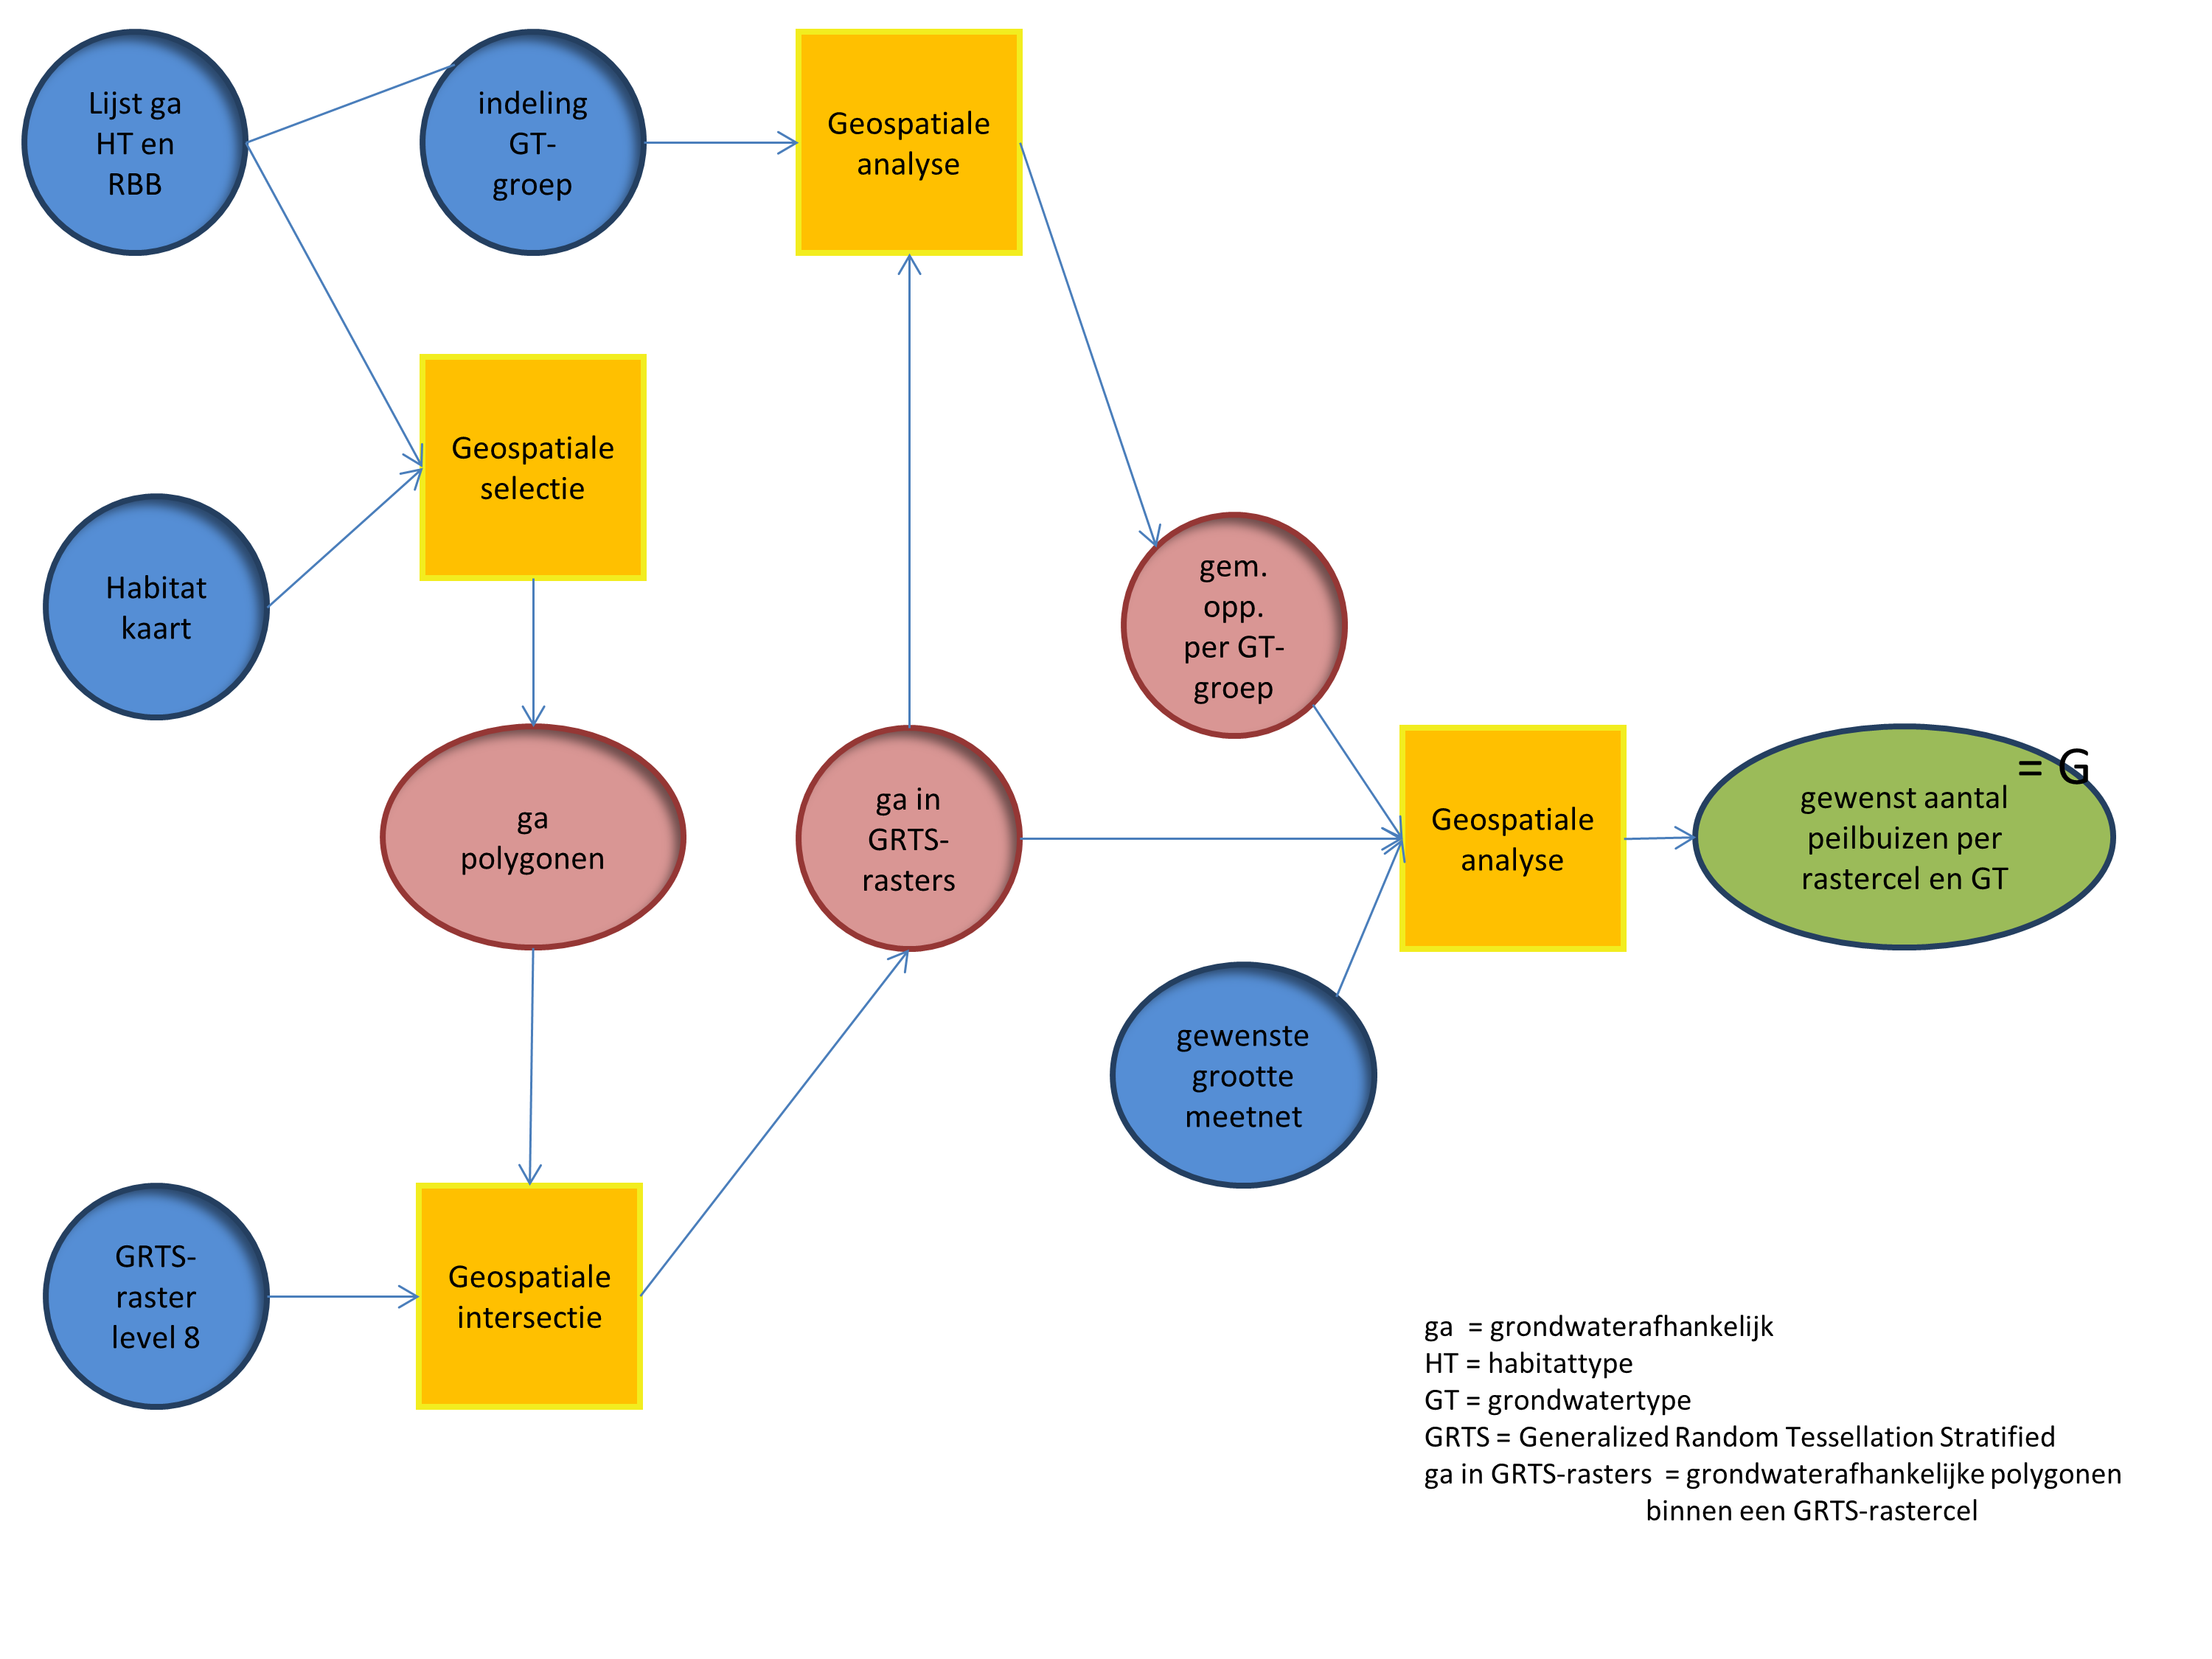
\includegraphics[width=10in]{figures/workflow_rasterselectie} \caption{werkgang selectie rastercellen. Blauw
gekleurde cirkels zijn brongegevens. De rode gekleurde zijn genereerde
data. Het groen gekleurde is een (tussentijds) output-resultaat. De gele
vakken stellen handelingen/bewerkingen voor.}\label{fig:workflow-rastercellen}
\end{figure}

\subsection{Selectie van de
meetpunten}\label{selectie-van-de-meetpunten}

In dit deel bespreken we hoe we aan de gekozen rastercellen effectief
meetpunten kunnen koppelen. Een meetpunt is een locatie waar het
(freatisch) grondwaterpeil periodiek gemeten wordt (of zal worden). In
de praktijk gebeurt dat in een piëzometer of peilbuis.\footnote{Normaal
  gesproken duidt in dit rapport de term meetpunt op de locatie eerder
  dan op het meetinstrument (peilbuis of piëzometer), maar soms slaat
  het op beide. Met peilbuis wordt in dit document ook een piëzometer
  bedoeld.}

Elke locatie die tot één van de GT-groepen behoort, kan in principe in
het meetnet opgenomen worden. Locaties waarvan het onduidelijk is tot
welke GT-groep ze behoren worden niet meegenomen. Dit kunnen locaties
zijn die op grens liggen van habitatvlekken die tot een verschillende
GT-groep behoren of het zijn locaties die in een habitatvlek gelegen
zijn dat gekarteerd is als een complex van vegetaties die tot
verschillende GT-groepen behoren. In de praktijk wordt deze voorwaarde
toegepast door enkel die habitatvlekken en/of peilbuizen te selecteren
die voor 50\% of meer toegewezen kunnen worden aan eenzelfde GT-groep en
die op minstens 3 m afstand liggen van een andere GT-groep.

Figuur \ref{fig:workflow-selectiepb-part1} geeft een schematisch
overzicht van de werkgang die gevolgd werd om na te gaan welke
peilbuizen beschikbaar zijn.




\begin{figure}
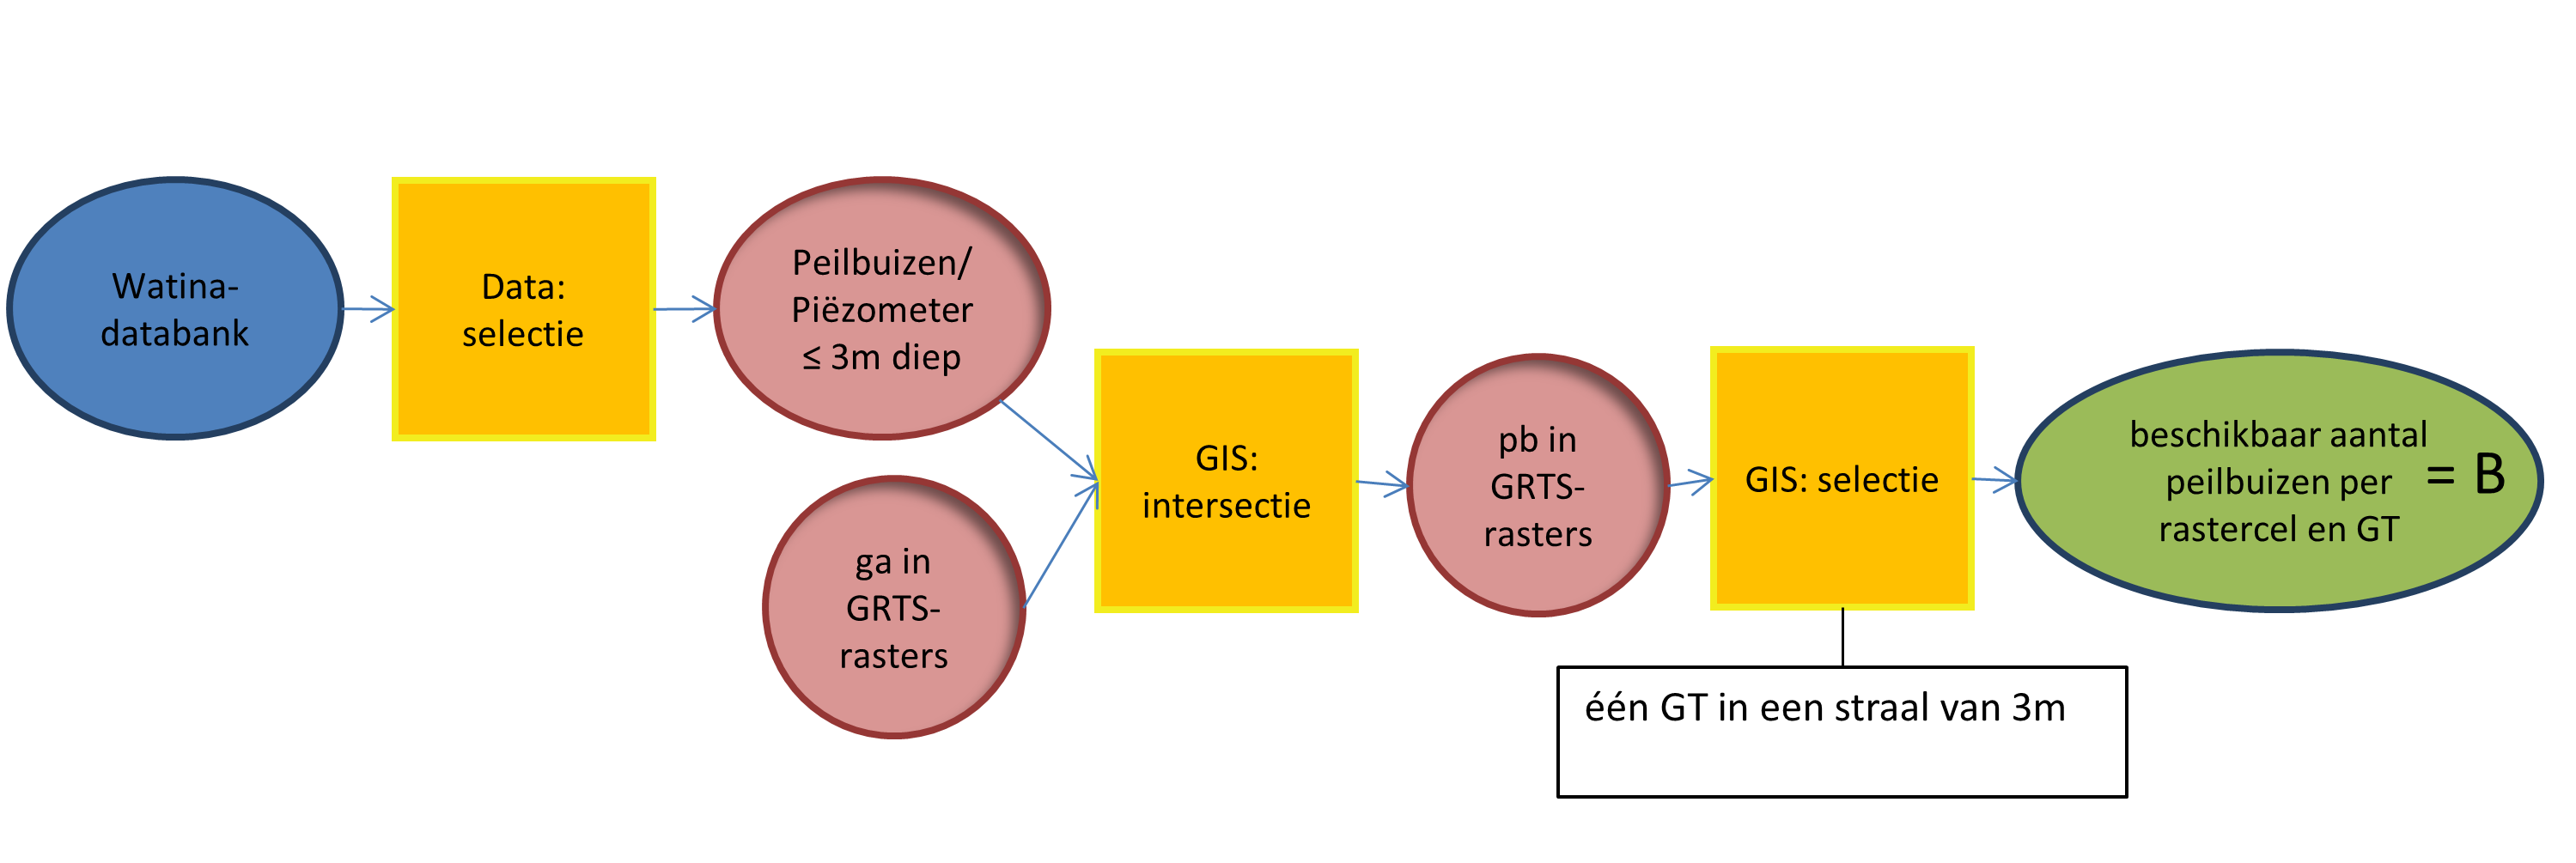
\includegraphics[width=10in]{figures/workflow_pbselectie_part1} \caption{werkgang selectie rastercellen. Voor de
betekenis van de symbolen zie figuur \ref{fig:workflow-rastercellen}.}\label{fig:workflow-selectiepb-part1}
\end{figure}

\subsubsection{Indeling van rastercellen in
categorieën}\label{indeling-cat}

We willen de toewijzing van een meetpunt aan een rastercel afhankelijk
stellen van de verhouding tussen het aantal meetpunten dat voor een
rastercel gezocht wordt (zie hoger) en het aantal effectief beschikbare
meetpunten met een peilbuis.

We willen er ook rekening mee houden dat een beschikbaar meetpunt niet
noodzakelijk ook een geschikt meetpunt is.

Afhankelijk van die verhoudingen worden de \emph{rastercellen}
\textbf{per GT-groep} eerst in categorieën ingedeeld. Deze opdeling is
een hulp bij het ontwerp, omdat elke categorie een specifieke
behandeling vraagt.

\emph{A. Alle meetpunten met een peilbuis zijn kwalitatief
gelijkwaardig}

We stellen eerst voor de eenvoud dat alle beschikbare meetpunten even
geschikt zijn: er wordt bvb. geen onderscheid gemaakt tussen een lang en
een kort bemeten meetpunt. Vergelijken we dan de vraag, het gewenste
aantal meetpunten per rastercel (= G), met het aanbod van meetpunten met
een peilbuis (of kortweg het aantal peilBuizen = B) dan kunnen de
rastercellen in drie categorieën verdeeld worden. De categorieën sluiten
elkaar mutueel uit.

\begin{itemize}
\tightlist
\item
  Cat. 1: de vraag is groter dan het aanbod (G \textgreater{} B)
\end{itemize}

Er zijn geen meetpunten met een peilbuis of er is een gebrek aan.

\begin{itemize}
\tightlist
\item
  Cat. 2: de vraag is gelijk aan het aanbod (G = B)
\end{itemize}

Het aantal beschikbare meetpunten met een peilbuis stemt juist overeen
met het aantal dat gezocht wordt.

\begin{itemize}
\tightlist
\item
  Cat. 3: de vraag is kleiner dan het aanbod (G \textless{} B)
\end{itemize}

Er is een overschot aan meetpunten met een peilbuis.

\textbf{Categorie 1}

Vanuit het oogpunt van een meetnetontwerp kan een rastercel van
categorie 1 over twee soorten meetpunten beschikken. Je hebt meetpunten
zonder peilbuis en mogelijk ook meetpunten met een peilbuis. Specifiek
voor deze categorie is dat we op zoek willen gaan naar nieuwe
meetpunten. Voor de uitwerking van deze selectie van potentiële
geschikte habitatvlekken: zie paragraaf \ref{sel-pot-habvlek}.

Alle meetpunten die reeds een peilbuis hebben, worden zonder verdere
analyse geselecteerd.

\emph{\textbf{Bovenstaande is een voorstel. Je zou ook kunnen beslissen
dat enkel meetpunten met een peilbuis in aanmerking komen voor het
meetnet.}} \emph{\textbf{Of het tegenovergestelde is ook een
alternatief: dat voor de ruimtelijke balancering we geen voorkeur geven
aan meetpunten met een peilbuis en enkel rekening houden met het
voorkomen van geschikte (ttz behoren tot de gewenste GT-groep)
habitatvlekken.}} \emph{\textbf{We vinden dat het huidige voorstel een
goede balans vertoont tussen beide.}}

Het gaat hier vooral over een tijdsinvestering: dergelijke meetpunten
zullen pas na enkele jaren effectief kunnen meedraaien in het meetnet.
In afwachting daarvan zal het meetnet dus met een kleiner aantal
meetpunten moeten functioneren.

\textbf{Categorie 2}

De rastercellen van deze categorie zijn voor het meetnetontwerp een
zegen. Het aantal locaties met peilbuizen volstaat juist om te voldoen
aan de vraag. Alle locaties kunnen zonder verdere analyse in het meetnet
worden opgenomen.

\textbf{Categorie 3}

Voor een rastercel van categorie 3 stelt er zich een `luxe-probleem': er
is namelijk een overschot aan meetpunten met een peilbuis. Uit dit
aanbod moet nog het gewenste aantal meetpunten gekozen worden. Hiervoor
verwijzen we naar paragraaf \ref{sel-habvlek}.

\emph{B. De meetpunten met een peilbuis zijn kwalitatief niet
gelijkwaardig}

In werkelijkheid zijn niet alle meetpunten even geschikt.

De bovenstaande categorie-indeling blijft weliswaar behouden, maar er
zijn verschillen t.a.v. de selectie van meetpunten en het gebruik ervan
in het meetnet.

We noemen een meetpunt geschikt, indien er hiervoor een
droogte-indicator kan berekend worden. Het berekenen van deze indicator
op een meetpunt vergt een ononderbroken meetreeks van \emph{dagelijkse}
peilen en dit over een stabiele, langdurige periode (een paar tiental
jaren) . De beschikbare terreinwaarnemingen in Watina zijn hiervoor
meestal ontoereikend. Door middel van een tijdreeksanalyse (zie
\ref{tijdreeksanalyse}) kunnen de tijdreeksen met modelgegevens
aangevuld worden, waardoor het wel mogelijk wordt om de indicator te
berekenen.

Het zal bijgevolg op basis van de tijdreeksanalyse zijn dat meetpunten
als geschikt (een tijdsmodel is mogelijk) of niet geschikt (een
tijdsmodel is niet mogelijk) zullen bevonden worden. Deze evaluatie
willen we vertalen in het gebruik van het meetpunt in het meetnet. Een
geschikt meetpunt kan op basis van de data onmiddellijk in het meetnet
worden opgenomen. Een niet geschikt meetpunt daarentegen kan dat pas na
verloop van tijd, nl. wanneer er voldoende data zijn die toelaten een
betrouwbaar tijdreeksmodel (zie onder) te bouwen.

Het vergt veel tijd om op alle beschikbare meetpunten een
tijdreeksanalyse uit te voeren. We willen dit beperken tot de
\emph{relatief (beschouwd op het niveau van combinatie rastercel en
GT-groep)} kwalitatief beste meetreeksen. Dit is een selectie, maar we
leggen geen absolute minimum-criteria op. Dit wil zeggen dat indien
bijvoorbeeld in een rastercel voor een bepaalde GT-groep de langste
tijdreeks één jaar is, dan zal deze peilbuis toch voor een
tijdreeksanalyse geselecteerd kunnen worden. De kans wordt uiteraard
kleiner dat met deze beperkte data een betrouwbaar model kan gebouwd
worden.

We delen de meetpunten daarom op in een aantal kwaliteitsklassen op
basis van volgende
\textbf{\protect\hypertarget{basiskwaliteitscriteria}{}{basiskwaliteitscriteria}}
:

\begin{enumerate}
\def\labelenumi{(\arabic{enumi})}
\item
  De meetpunten hebben vanaf 2000 voor minstens één jaar een goede
  tijdreeks\footnote{Een kwalitatief goed meetjaar wordt hier
    gedefinieerd als een hydrologisch jaar waarvoor een lg3 kan berekend
    worden. Dit houdt in dat er minstens 20 goed gespreide metingen per
    jaar zijn. Het verschil tussen twee metingen mag niet groter zijn
    dan 30 dagen en de eerste en laatste meting moet resp. in april en
    maart (van het daaropvolgende kalenderjaar) vallen. lg3 = het
    gemiddelde van de drie laagste waterpeilen binnen een hydrologisch
    jaar (1 april - 31 maart), waarbij er tussen deze drie metingen
    minstens 14 dagen verschil ligt. --\textgreater{}}, die een toelaat
  een zogenaamde lg3-waarde\footnote{Een kwalitatief goed meetjaar wordt
    hier gedefinieerd als een hydrologisch jaar waarvoor een lg3 kan
    berekend worden. Dit houdt in dat er minstens 20 goed gespreide
    metingen per jaar zijn. Het verschil tussen twee metingen mag niet
    groter zijn dan 30 dagen en de eerste en laatste meting moet resp.
    in april en maart (van het daaropvolgende kalenderjaar) vallen. lg3
    = het gemiddelde van de drie laagste waterpeilen binnen een
    hydrologisch jaar (1 april - 31 maart), waarbij er tussen deze drie
    metingen minstens 14 dagen verschil ligt. --\textgreater{}} te
  berekenen.
\item
  Meetpunten met een \emph{recente} kwalitatief goede tijdreeks primeren
  boven meetpunten met een oudere tijdreeks.
\end{enumerate}

De meetpunten worden hierbij gerangschikt volgens aflopend jaartal
(eindjaar) van de laatst beschikbare kwalitatief goede tijdreeks.

Meetpunten worden als evenwaardig beschouwd als het verschil niet groter
dan \textbf{5} jaar is.

\begin{enumerate}
\def\labelenumi{(\arabic{enumi})}
\setcounter{enumi}{2}
\tightlist
\item
  Meetpunten met een \emph{langere} tijdreeks, t.t.z. een groter aantal
  kwalitatief goede meetjaren, krijgen ook een hogere prioriteit.
\end{enumerate}

Meetpunten waarvan het aantal niet meer dan \textbf{5} jaar van elkaar
verschilt, worden als evenwaardig beschouwd.

\begin{enumerate}
\def\labelenumi{(\arabic{enumi})}
\setcounter{enumi}{3}
\tightlist
\item
  Een meetpunt met een lange tijdreeks, maar niet recent, primeert op
  een meetpunt met een recentere maar
  \protect\hypertarget{derde-criterium}{}{kortere tijdreeks.}
\end{enumerate}

Deze basiskwaliteitscriteria zijn te beschouwen als een eerste screening
op basis van actueel beschikbare feitelijke grondwatermetingen.

Het gebruik van deze criteria leidt er ook toe dat in een rastercel bij
de toewijzing van een meetpunt, indien mogelijk (= in categorie 3),
rekening wordt gehouden met de datakwaliteit.

\textbf{\emph{vraag: wat te doen met bestaande meetlocaties die actueel
niet geschikt zijn? Worden deze weer geactiveerd (gevolgd in deze
versie) of geven we voorrang aan de ruimtelijke balans ?}}

\subsubsection{Tijdreeksanalyse}\label{tijdreeksanalyse}

Tijdreeksanalyse is een middel om grondwaterstandsmetingen te analyseren
(zie bijv. Von Asmuth \emph{et al.},
\protect\hyperlink{ref-RN877}{2004}). In feite zouden ook meetreeksen
van oppervlaktewaterpeilen geanalyseerd kunnen worden, maar dit is
weinig gebruikelijk, waarschijnlijk omdat er moeilijker een verband te
leggen is met het weer (zoals neerslag en verdamping). In dit project
willen we deze analysetechniek toepassen op grondwatermeetreeksen met
twee doeleinden:

\begin{itemize}
\tightlist
\item
  het verlengen of invullen van te korte of onregelmatige
  grondwaterstandsreeksen
\item
  het opsporen van lineaire trends
\end{itemize}

Het eerste doel is ook al hoger ter sprake gekomen. Slagen we er in om
op een betrouwbare wijze de waterstandsreeksen te
verlengen/vervolledigen, dan kan een meetpunt geschikt worden om in het
droogtemeetnet opgenomen te worden. De tijdreeksen krijgen ook een meer
uniforme lengte, waardoor het afleiden van een droogte-indicator meer
gestandaardiseerd wordt.

Het tweede doel is in feite een bijkomende selectiecriterium. Indien uit
een tijdreeksanalyse blijkt dat de waterstanden van een meetpunt
systematisch dalen of stijgen, leent dat meetpunt zich niet goed voor
het berekenen van een droogte-indicator. Met een systematische daling of
stijging bedoelen we een lineaire trend die niet door externe factoren
(opstuwen of graven greppels, waterwinning) kan verklaard worden. Indien
een tijdreeks een lineaire trend vertoont, wordt het meetpunt als
momenteel ongeschikt beschouwd.

Voor de tijdreeksanalyse doen we beroep op het computerprogramma
Menyanthes (KWR \& Waterware, \protect\hyperlink{ref-RN5899}{2018}).
Voor het samenstellen van de verklarende reeksen (neerslag en
evapotranspiratie) werd beroep gedaan op de data van de meetstations
beheerd door KMI, VMM, HIC en KNMI. Voor de waterstandgegevens werd de
Watina-databank geraadpleegd.

Er werden, zoals hoger al aangehaald, geen kwaliteitseisen gesteld aan
een meetreeks die deze a priori zou uitsluiten van een tijdreeksanalyse.
Het is, door het hoge aantal beschikbare meetpunten, echter niet
doenbaar om een tijdreeksanalyse uit te voeren op alle meetpunten.

Wel werden alle meetreeksen van de meetpunten die behoren tot
rastercellen van cat. 1 en cat. 2 geanalyseerd. Voor categorie 3 bleef
dat beperkt tot die meetpunten die behoren tot de hoogste
kwaliteitsklassen die nodig zijn om tot het gewenst aantal meetpunten te
komen.

Een meetreeks werd weerhouden als er een tijdsmodel kon voor
samengesteld worden dat minstens 66\% van de variatie in de waargenomen
peilen (cfr. EVP, explained variance percentage, in de
Menyanthes-software) kon verklaren en ook geen significante lineaire
trend vertoont. Bij het tijdsmodel werden uitsluitend neerslag- en
evapotranspiratiedata als verklarende reeksen gebruikt.

Minstens twee derden van het peilverloop dient dus verklaard te kunnen
worden door het weer. Eén derde kan/mag door andere factoren beïnvloed
worden (bijv. het naburige peil van een waterloop).

Een \protect\hypertarget{lintrend}{}{lineaire trend} werd als
significant beschouwd indien de stijging/daling per jaar (=
\texttt{trend}), rekening houdend met de standaardafwijking hierop (=
\texttt{se}), voldoet één van de volgende twee regels:

\[trend - 1.96* se > 1(cm/jaar)\] of \[trend + 1.96* se < -1(cm/jaar)\]
Er is dan 2.5\% kans een trendwaarde die groter resp. kleiner is ten
onrechte als een significante trend te bestempelen.

De kwaliteit van een tijdreeks kan na een tijdreeksanalyse anders
beoordeeld worden. Bijvoorbeeld een meetpunt met veel peilmetingen, die
echter een duidelijke lineaire trend vertonen, is weinig geschikt om
onmiddellijk in het meetnet te worden opgenomen. Anderzijds komt een
meetpunt met minder metingen, maar waarvoor een goed model kan gebouwd
worden (zonder lineaire trend), wel in aanmerking om nu reeds in het
meetnet te worden opgenomen.

Bij de modelselectie kwam toch ook nog expertoordeel bij kijken.

De gestelde kwaliteitseisen leiden niet tot uitsluiting van een
tijdreeksanalyse. In principe kan elke peilbuis, zelfs al is er maar één
meting van bekend, geselecteerd worden. En zo geschiedde ook. Deze
meetreeksen werden manueel afgekeurd. Sommige heel korte tijdreeksen
hadden zelfs bijna een perfecte fit, maar het was toch onbetrouwbaar om
hiermee waarden te simuleren over een relatief lange tijdsperiode.

Anderzijds werd een model met een verklarende variantie beneden 66\%
soms nog weerhouden, indien bleek dat het model de lage
grondwaterstanden goed kon modelleren.

Een lange tijdreeks met een trend \textless{} 1cm/jaar, maar waarbij de
peilen maar weinig schommelen (kleine amplitude) kon toch owv deze trend
afgekeurd worden (bijv. een tijdreeks waarbij over 15 jaar er een
duidelijke stijging van 10 cm te zien is, terwijl de peilen slechts een
amplitude van 40 cm hebben) en vice versa.

Het al dan niet weerhouden van een tijdreeks kan in categorie 3 gevolgen
hebben voor het selecteren van een meetpunt. Immers hierbinnen wordt
gestreefd minstens zoveel geschikte meetpunten te vinden dan er gezocht
worden. Zijn er meer geschikte punten dan gezocht, dan kan gestopt
worden met verder zoeken. Zolang dit aantal echter niet bereikt is,
wordt (iteratief) verder gezocht.

\subsubsection{Bijkomende GRTS-analysen}\label{bijkomende-grts-analysen}

Afhankelijk van de verhouding tussen het aantal gewenste, beschikbare
enerzijds (categorie 1) en het aantal gewenste en geschikte peilbuizen
anderzijds (categorie 3), moeten er nog enkele bijkomende GRTS-analysen
uitgevoerd worden.

\paragraph{Selecteren van potentiële geschikte habitatvlekken voor
rastercellen waarvoor er te weinig peilbuizen bestaan (cat.
1)}\label{sel-pot-habvlek}

Voor rastercellen van cat. 1 is er een nood aan één of meer extra
meetpunten. Om hierbinnen (8192 * 8192 m) de plaatskeuze zo aselect
mogelijk te doen, doen we beroep op het fijnste GRTS-raster
`GRTSmaster\_habitats' (celgrootte = 32 m). Opnieuw wordt op deze manier
een synergie bekomen met de aselecte locatiekeuzes in MNM. Elk
deelrastercel heeft binnen de rastercel een bepaalde rangnummer. Alleen
deelrastercellen \emph{die voor het merendeel vegetaties bevatten die
tot de GT-groep behoren} komen voor selectie in aanmerking. De
deelrastercel(len) met het /de laagste rangnummer(s) zal/zullen dan
geselecteerd worden. Aan de selectie van deelrastercellen kunnen, naast
de aanwezigheid van de juiste GT-groep, nog bijkomende voorwaarden
gekoppeld worden (beheerder, \ldots{}). Blijkt bij inspectie op terrein
dat de geselecteerde plaats toch niet aan de verwachtingen/criteria
voldoet, dan wordt binnen dezelfde rastercel de rastercel die het eerst
in rang volgt binnen een zoekstraal van 1 km bezocht.

\paragraph{Selecteren van een meetpunt in een rastercel waarvoor
meerdere kandidaten zijn (cat. 3)}\label{sel-habvlek}

Afhankelijk van de verhouding tussen gewenste aantal en het aantal
geschikte peilbuizen is er mogelijk een extra analyse nodig.

\begin{itemize}
\item
  Is het aantal geschikte peilbuizen groter dan wordt enkel binnen deze
  groep een GRTS-analyse uitgevoerd om het gewenste aantal te
  selecteren.
\item
  Is het aantal kleiner dan wordt er uit alle beschikbare peilbuizen via
  een GRTS-analyse het gewenste aantal geselecteerd.
\item
  Is het aantal gelijk dan hoeft er geen verdere analyse te gebeuren.
  Alle meetpunten kunnen in het meetnet worden opgenomen.
\end{itemize}

Net zoals voor cat. 1 willen we de keuze zo aselect mogelijk doen. We
doen hiervoor terug beroep op het fijnste GRTS-raster
`GRTSmaster\_habitats' (celgrootte = 32 m). Het/de meetpunt(en) gelegen
in de deelrastercel(len) met het /de laagste rangnummer(s) zal/zullen
dan geselecteerd worden. Deze werkwijze laat ook gemakkelijk toe om
reserve-punten te kiezen. Het zijn de meetpunten die in rang volgen op
de laagste rang van een gekozen punt.

\subsubsection{Samenvatting werkgang selectie
peilbuizen}\label{samenvatting-werkgang-selectie-peilbuizen}

Na de ruimtelijke selectie weten we hoeveel meetpunten er per rastercel
en per GT-groep gewenst zijn.

We proberen die wensen zoveel mogelijk in te vullen met bestaande
peilbuizen waarvan hun meetreeksen toelaten een droogte-indicator te
berekenen.

Hiertoe evalueren we de kwaliteit van de meetreeksen op basis van de
mogelijkheid om voor minstens één jaar een lg3 te berekenen voor de
metingen na 2000, van het aantal meetjaren en van de ouderdom van de
meetreeks.

De kwalitatief beste meetreeksen worden verder beoordeeld met een
tijdreeksanalyse. Door het grote aantal peilbuizen was het niet mogelijk
ze alle te analyseren. De voorkeur ging daarom uit naar de relatief
beste reeksen. Een meetreeks wordt `geschikt' bevonden als minstens 2/3
van de variatie door het weer kan verklaard worden en er in de reeks
geen lineaire trend te zien is. Op basis van de tijdreeksanalyse worden
de meetreeksen geherklasseerd in `geschikt', `niet 'geschikt' en
`onbekend' (indien niet behandeld). Er worden minstens zoveel peilbuizen
geanalyseerd tot er evenveel of meer geschikte reeksen zijn dan het
gewenste aantal, zoniet worden ze allemaal geanalyseerd.

Is een meetreeks `geschikt', dan kan de peilbuis onmiddellijk in het
meetnet opgenomen worden. Is ze `niet geschikt', dan kan dit pas na
verloop van enkele jaren.

De rastercellen kunnen in drie categorieën (cat. 1- 3) verdeeld worden
op basis van de verhouding tussen het aantal gewenste en beschikbare
peilbuizen. Bij cat. 1 zijn er te weinig peilbuizen. De meetreeksen van
alle peilbuizen werden geanalyseerd. Via een GRTS-procedure wordt het
ontbrekend aantal aangevuld met habitatvlekken. In cat. 2 klopt het
gewenste aantal met het beschikbaar aantal en hoeft er geen aansluitende
analyse meer uitgevoerd te worden.

In cat. 3 zijn er meer peilbuizen beschikbaar. Afhankelijk van de
verhouding tussen het gewenste aantal en het aantal geschikte peilbuizen
is er mogelijk een extra GTRS-analyse nodig om het gewenste aantal te
selecteren.

Figuur \ref{fig:workflow-selectiepb-part2} geeft schematisch het
overzicht van de werkgang die gevolgd werd om uit de beschikbare
peilbuizen meetpunten te selecteren en deze desnoods aan te vullen met
nieuwe.




\begin{figure}
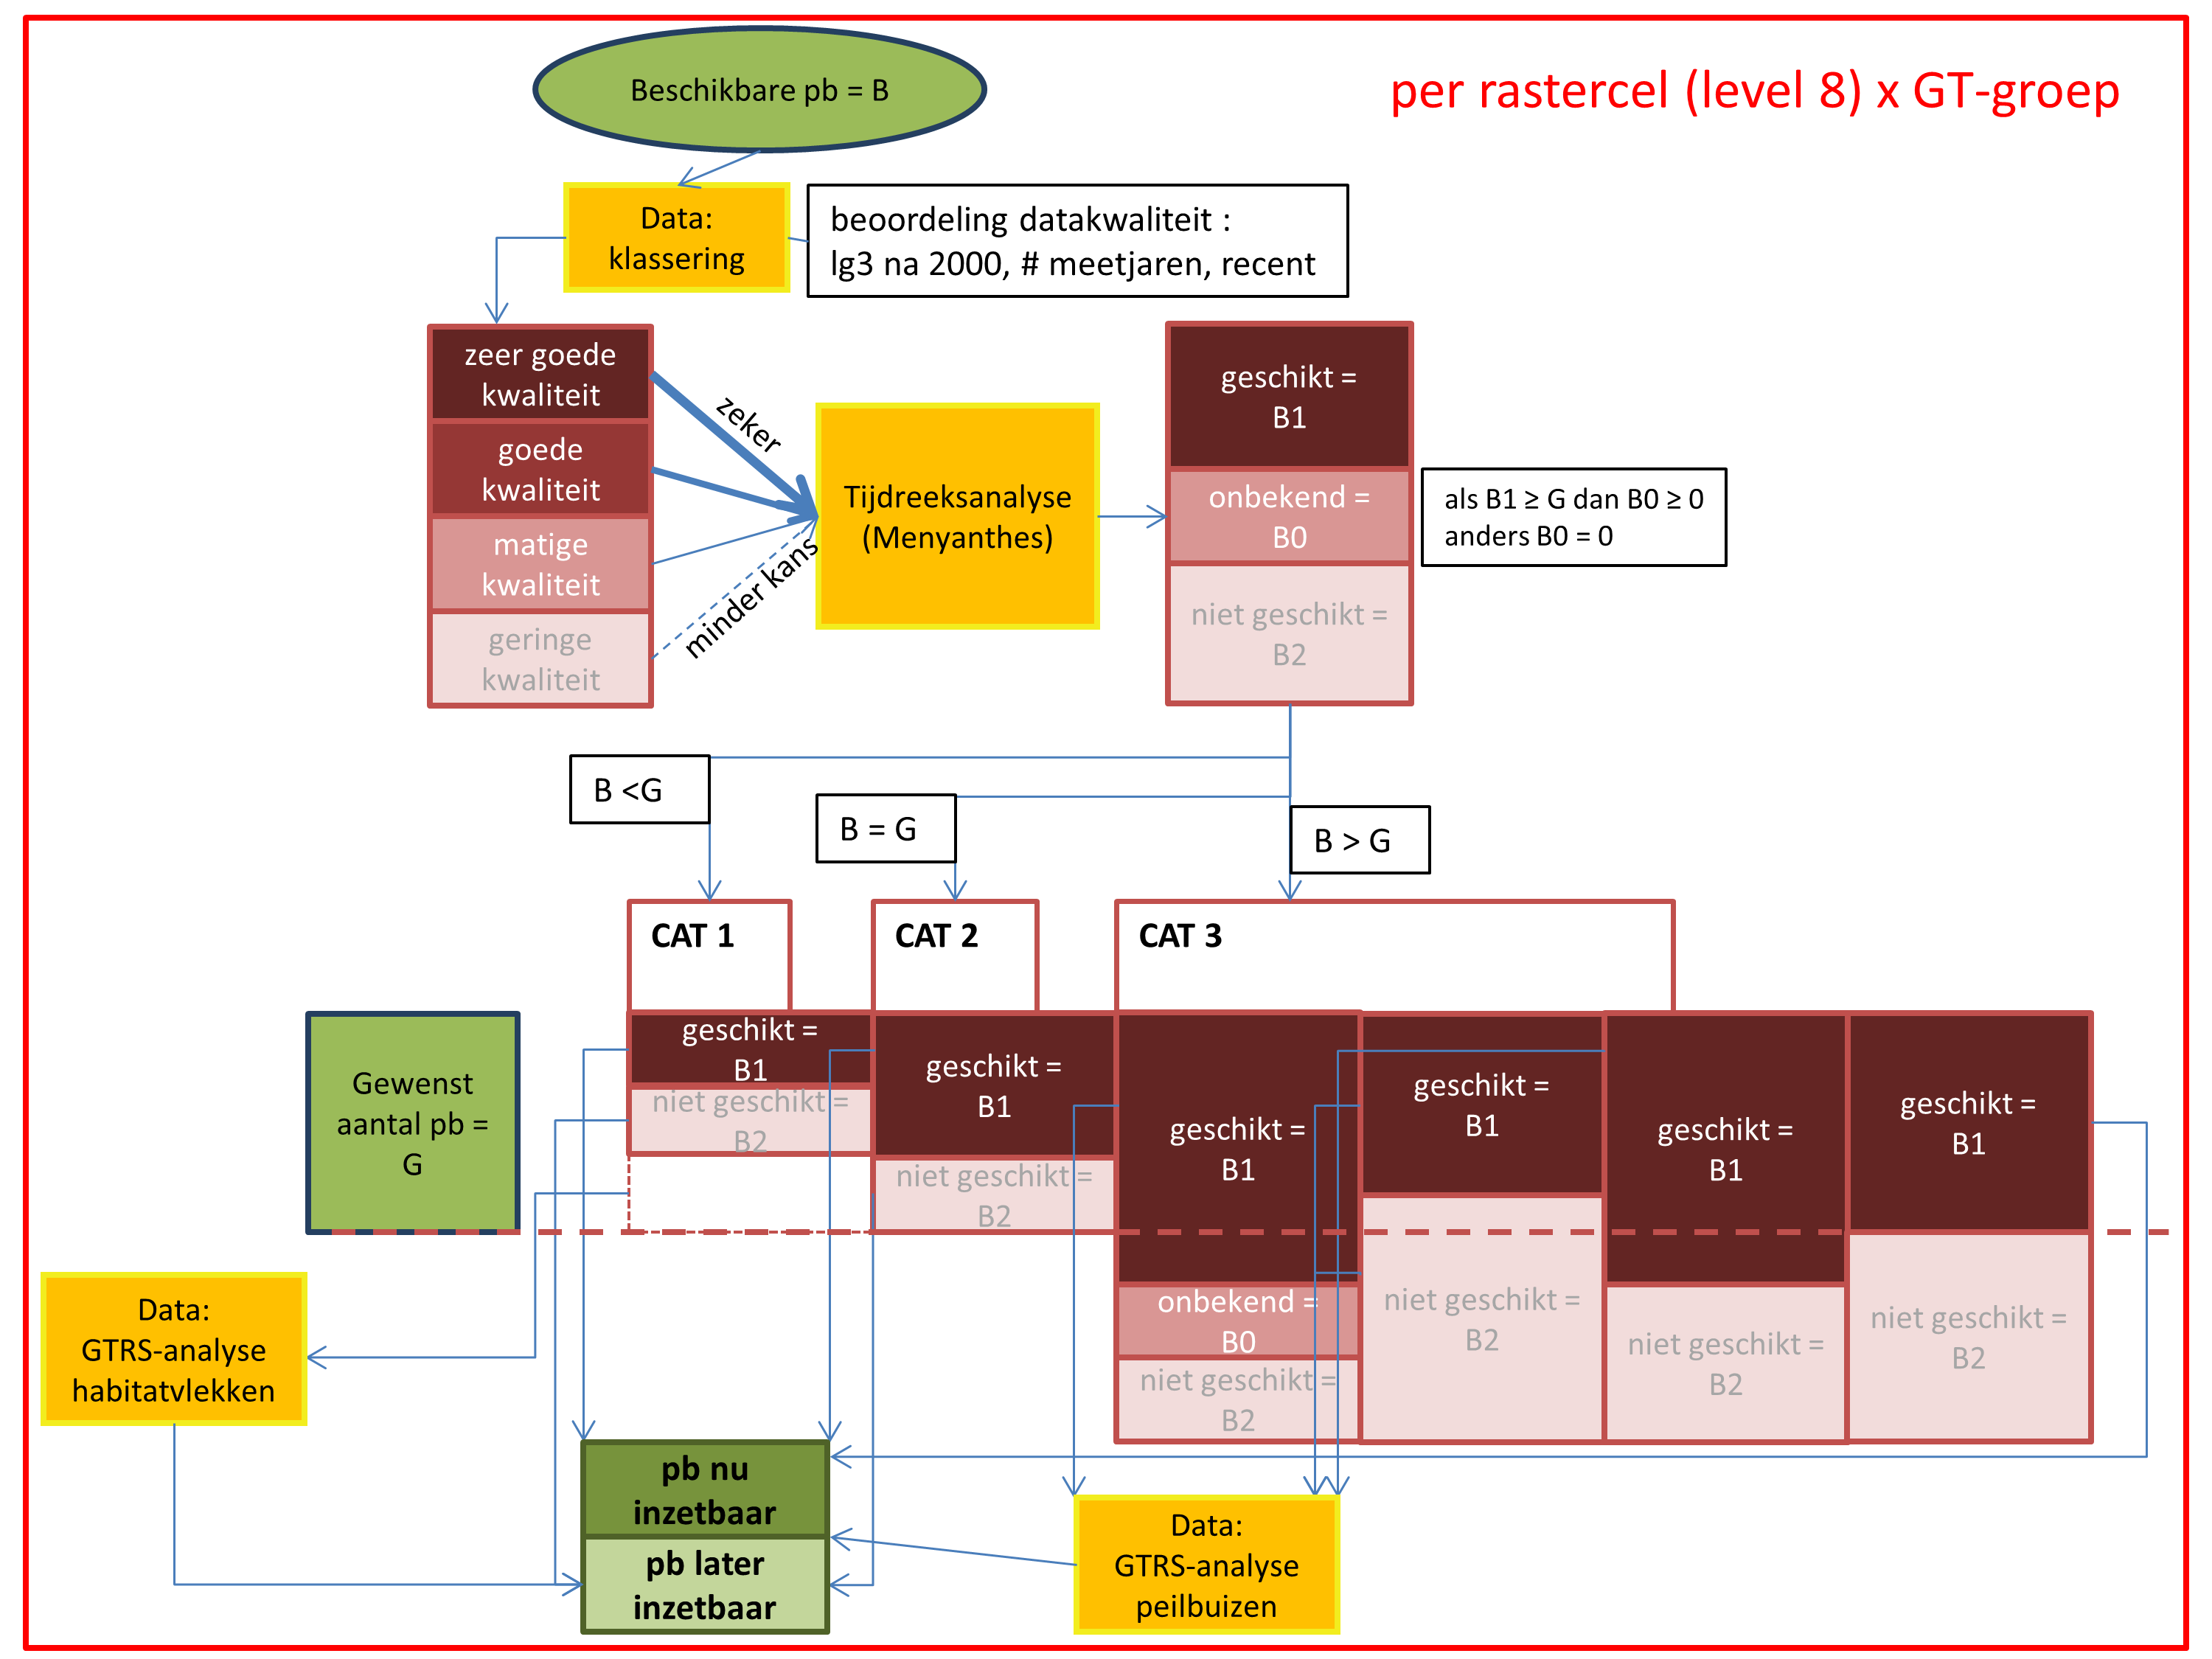
\includegraphics[width=10in]{./figures/workflow_pbselectie_part2} \caption{werkgang selectie rastercellen. Voor de
betekenis van de symbolen zie figuur \ref{fig:workflow-rastercellen}.}\label{fig:workflow-selectiepb-part2}
\end{figure}

\section{Bepaling droogte-indicator voor de geselecteerde
punten}\label{bepaling-droogte-indicator-voor-de-geselecteerde-punten}

\subsection{Droogte-indicatoren}\label{droogte-indicatoren}

Er zijn verschillende indicatoren mogelijk om droogte te detecteren
(Wouters \emph{et al.}, \protect\hyperlink{ref-RN5703}{2018}).

Binnen dit project berekenen we de huidig gebruikte droogte-indicator:
De indicator vergelijkt de grondwaterstand op een gegeven dag met de
grondwaterstanden die op diezelfde plaats en dag van het jaar zijn
voorgekomen in het verleden. De indicator evalueert dus de
droogtetoestand rekening houdend met de tijd van het jaar. Zo kunnen ook
relatief lage grondwaterstanden in het voorjaar als droogte aangeduid
worden.

De indicator kleurt respectievelijk rood, oranje of geel op een bepaalde
plaats en dag zodra de grondwaterstand er minstens 14 dagen onder de
p10, p20 of p30 (situatie met overschrijdingskans van 10, 20 of 30\%) is
gebleven. \emph{\textbf{De indicator kleurt respectievelijk rood, oranje
of geel voor Vlaanderen als minstens de helft van de putten kleurcode
rood, oranje of geel heeft. (vraag: is dit ook aangewezen voor dit
meetnet ?). }} \emph{\textbf{Een opsplitsing per bekken hadden we
tijdens de eerste vergadering niet weerhouden.}}

\subsection{Berekeningswijze voor de geselecteerde
punten}\label{berekeningswijze-voor-de-geselecteerde-punten}

Voor het berekenen van de droogte-indicator doen we beroep op
tijdreeksen van \textbf{\emph{minimaal 20 (of meer?) jaren lang}}, al
dan niet gemodelleerde, metingen en waarbij metingen van 2017 en 2018
uitgesloten werden. Het is namelijk nu nog onduidelijk of de actuele
vegetatie geen nadelige effecten van deze twee droge zomers heeft gekend
(door naijling). Voor elke bestaande geselecteerde meetlocatie wordt dan
voor elke dag van het jaar (\textbf{\emph{vraag: of alleen voor het
groeiseizoen: 1 april - 1 oktober? }}) de p10, p20 en p30
percentielwaarde berekend.

\hypertarget{refs}{}
\hypertarget{ref-RN5899}{}
KWR \& Waterware (2018). Menyanthes, versie 3.x.b.w.

\hypertarget{ref-onkelinx_grts_2019}{}
Onkelinx T., Westra T. \& Vanderhaeghe F. (2019). GRTS master sample for
habitat monitoring in Flanders. DOI:
\url{https://doi.org/10.5281/zenodo.2682323}.

\hypertarget{ref-vanderhaeghe_grtsmh_diffres_2019}{}
Vanderhaeghe F. (2019). GRTSmh\_diffres: The raster data source
GRTSmaster\_habitats converted to 9 hierarchical cell address levels at
the corresponding lower resolution. DOI:
\url{https://doi.org/10.5281/zenodo.3354406}.

\hypertarget{ref-vanderhaeghe_meetnetten_2018}{}
Vanderhaeghe F., Van Calster H., Onkelinx T. \& Westra T. (2018).
Meetnetten Natuurlijk Milieu: Steekproefopzet en inferentiestrategie.
Conceptrapport. Instituut voor Natuur- en Bosonderzoek, Brussel. URL:
\url{https://drive.google.com/open?id=1OlLCdEAvWOelzXeTytqsuKfcw7B3HQov}.

\hypertarget{ref-RN877}{}
Von Asmuth J., Maas K. \& Cirkel G. (2004). Tijdreeksanalyse van
grondwaterstanden nu binnen ieders bereik. H 2 O 24: 31--33. URL:
\url{https://drive.google.com/open?id=0B7K_7SGyjAgMbzlSYmdNb2FWQkE}.

\hypertarget{ref-RN5703}{}
Wouters J., Denys L. \& Vanden Borre J. (2018). Advies over
droogte-indicatoren voor grondwaterafhankelijke vegetaties en
stilstaande wateren met belangrijke natuurwaarden. Adviezen van het
instituut voor natuur- en bosonderzoek. Instituut voor Natuur- en
Bosonderzoek, Brussel.


\end{document}
